% !TeX encoding = UTF-8
% 
% 作者: 李永建 澳门科技大学-毕业论文latex模板-2023
% Github: https://github.com/iihciyekub/MUST-Thesis
% Overleaf(read): https://www.overleaf.com/read/mjzpcxztzqzv
% 最后更新: 2023-03-18

\documentclass[
    添加扉页=是,
    添加原創聲明頁=是,
    添加校徽水印=是,
    奇偶页邊距對稱=不,
]{.def/must}


% 论文基本信息,必填不能删除
\def\shool              {澳門科技大學}
\def\cntitle            {XXX 銀行(澳門分行)與 XXX 銀行合併之研究}
\def\entitle            {The Study of XXX Bank (Macau Branch) Merged the XXX Bank in Macao}
\def\Name               {XXX}% 名稱
\def\StudentNo          {1809853G-BM30-0053}% 學號
\def\Faculty 	        {XXX 學院}% 所在學院
\def\Program 	        {XXXX}% 課程名稱
\def\Major              {XXXX}% 專業名稱
\def\Supervisor	        {XXXX}% 指導老師
\def\DateofWriting		{\datea\today}% 設置論文寫作完成時間
\def\DateofDeclaration	{\dateb\today}% 設置論文原創聲明時間
\def\DateofSignature	{2023/06/30}% 設置簽署論文原創聲明的時間
\def\PublicAfterYears   {5}% 設置論文幾年后公開




 
\begin{document}

\begin{abstract@cn}{關鍵字1、關鍵字1、關鍵字1、關鍵字1、}
本研究採用2009 年至2014 年首度上市的公司279 家為研究
樣本,檢驗公司治理與財務績效之關聯性。利用樣本公司上市時
的公司治理變數,檢驗公司治理對上市後的會計績效影響與上市
後30 天的市場報酬,再進而依據過去文獻對公司治理變數的論
述,以單一指標衡量,依研究對象中位數區分公司治理程度,以
及公司治理變數給予不同分數,驗證對財務績效之影響,並比較
「有價證券上市審查準則」強化公司治理制度前後之上市公司,
在公司治理與財務績效上是否有差異。透過相關分析、T 檢定、
迴歸分析,檢驗三大研究假說,實證結果獲得以下主要結論:
本研究採用2009 年至2014 年首度上市的公司279 家為研究
樣本,檢驗公司治理與財務績效之關聯性。利用樣本公司上市時
的公司治理變數,檢驗公司治理對上市後的會計績效影響與上市
後30 天的市場報酬,再進而依據過去文獻對公司治理變數的論
述,以單一指標衡量,依研究對象中位數區分公司治理程度,以
及公司治理變數給予不同分數,驗證對財務績效之影響,並比較
「有價證券上市審查準則」強化公司治理制度前後之上市公司,
在公司治理與財務績效上是否有差異。透過相關分析、T 檢定、
迴歸分析,檢驗三大研究假說,實證結果獲得以下主要結論:
本研究採用2009 年至2014 年首度上市的公司279 家為研究
樣本,檢驗公司治理與財務績效之關聯性。利用樣本公司上市時
的公司治理變數,檢驗公司治理對上市後的會計績效影響與上市
後30 天的市場報酬,再進而依據過去文獻對公司治理變數的論
述,以單一指標衡量,依研究對象中位數區分公司治理程度,以
及公司治理變數給予不同分數,驗證對財務績效之影響,並比較
「有價證券上市審查準則」強化公司治理制度前後之上市公司,
在公司治理與財務績效上是否有差異。透過相關分析、T 檢定、
迴歸分析,檢驗三大研究假說,實證結果獲得以下主要結論:
本研究採用2009 年至2014 年首度上市的公司279 家為研究
樣本,檢驗公司治理與財務績效之關聯性。利用樣本公司上市時
的公司治理變數,檢驗公司治理對上市後的會計績效影響與上市
後30 天的市場報酬,再進而依據過去文獻對公司治理變數的論
述,以單一指標衡量,依研究對象中位數區分公司治理程度,以
及公司治理變數給予不同分數,驗證對財務績效之影響,並比較
「有價證券上市審查準則」強化公司治理制度前後之上市公司,
在公司治理與財務績效上是否有差異。透過相關分析、T 檢定、
迴歸分析,檢驗三大研究假說,實證結果獲得以下主要結論:
\end{abstract@cn}

\begin{abstract@en}{keyword1、keyword1、keyword1、keyword1、}
This research used 279 companies established between 2009 and 2014 as the
sample, examining the relationship between corporate governance and financial
performance. Corporate governance variable during the time when company
gets started is used to examine the effect of corporate governance on accounting
effectiveness after the company has been on the market, as well as the effect on
the return rate during the first 30 days of the company’s opening. Further
analysis from literature review on corporate governance, using single
measurement, is according to the median of the level of corporate governance
and the rating of corporate governance variable, to cross examine its effect on
financial performance. Also, a comparison of the effect on strengthening
corporate governance using “Stock Exchange Listing Standards” before and
after the company was listed on the stock market on corporate governance and
financial performance. Correlation, T-test, and Regression analysis were used to
examine three hypotheses. Findings include: 
\begin{enumerate}[leftmargin=1.2 em,label=\arabic*) ]
    \item  Company characteristics
High Tech industry has better corporate governance mechanism than traditional
industries.
    \item  Characteristic of corporate governance level
High corporate governance companies have better accounting effectiveness and
market performance.
    \item  Correlation between economic cycle and industry type v.s. corporate
 governance and management effectiveness
Industry characteristics will reinforce the impact of corporate governance level
towards accounting effectiveness; whereas economic cycle will reinforce the
impact of corporate governance level toward market effectiveness.
    \item  In a time of recession, corporate governance showed positive effect on
market effectiveness.
    \item  Corporate governance has a positive correlation with accounting
effectiveness when there were fewer diversified investors; with the
exception of high tech industry, which shows positive correlation between
corporate governance level and accounting effectiveness when there were
more diversified investors.
    \item  Companies participated in strengthening corporate governance since the
policy was enforced showed positive relationship with management
effectiveness.
    \item  Better corporate governance and management effectiveness since the
legislation was enforced.
    \item  Corporate governance is stronger among the high tech industry. 
\end{enumerate}
This research used 279 companies established between 2009 and 2014 as the
sample, examining the relationship between corporate governance and financial
performance. Corporate governance variable during the time when company
gets started is used to examine the effect of corporate governance on accounting
effectiveness after the company has been on the market, as well as the effect on
the return rate during the first 30 days of the company’s opening. Further
analysis from literature review on corporate governance, using single
measurement, is according to the median of the level of corporate governance
and the rating of corporate governance variable, to cross examine its effect on
financial performance. Also, a comparison of the effect on strengthening
corporate governance using “Stock Exchange Listing Standards” before and
after the company was listed on the stock market on corporate governance and
financial performance. Correlation, T-test, and Regression analysis were used to
examine three hypotheses. Findings include:
\end{abstract@en}


% 添加目录 
\addtableofcontents





\chapter{緒論}


\section{研究動機與目的}
\subsection{研究動機}
\par 美國學者對公司治理的討論可追溯自1930 年代,Berle \&
Means(1932)指出,美國企業存在著股權分散的必要性,因為隨著企
業規模不斷的擴大,使得多數的中大型公司皆需將經營權與所有權
加以分離來經營,以期達到專業化的目的。
\par 有系統地討論此一問題者為Jensen,在1988 年Jensen 首度有系統地
收錄以公司治理為主題的文章(Weston, Siu \& Johnson; 2002)。

\noindent 公式:式子置中,編號靠右,如
\begin{equation}
V_0=X_0(1-T)(1-b) \sum_{t=1}^n \frac{(1+g)^t}{(1+k)^t}+\frac{X_0(1-T)(1-g)^{n+1}}{k(1+k)^n}
\end{equation}


\par 美國學者對公司治理的討論可追溯自1930 年代,Berle \&
Means(1932)指出,美國企業存在著股權分散的必要性,因為隨著企
業規模不斷的擴大,使得多數的中大型公司皆需將經營權與所有權
加以分離來經營,以期達到專業化的目的。
$V_0=X_0(1-T)(1-b) \sum_{t=1}^n \frac{(1+g)^t}{(1+k)^t}+\frac{X_0(1-T)(1-g)^{n+1}}{k(1+k)^n}$ 
有系統地討論此一問題者為Jensen,在1988 年Jensen 首度有系統地
收錄以公司治理為主題的文章(Weston, Siu \& Johnson; 2002)。
\begin{enumerate}
\item 第一个枚举第一个枚举第一个枚举第一个枚举第一个枚举第一个枚举第一个枚举第一个枚举第一个枚举第一个枚举第一个枚举第一个枚举第一个枚举 
\item 第二个枚举 
\item 第三个枚举 
\end{enumerate}

% 添加表格
\begin{table}[htbp]
    \centering
    \caption{My Table}
    \label{tab:mytable}
    \csvautobooktabular{data.csv} 
\end{table}




\begin{sidewaystable}[!htp]
	\caption{示例旋轉長表} 
	\centering
	\setlength{\tabcolsep}{10mm}
	\begin{tabular}[l]{@{}lcccccc}		
	\toprule		
	Class$^{\rm a}$ & $\gamma_1$ & $\gamma_2$$^{\rm b}$& $\langle \gamma \rangle$& $G$ & $|{ f}|$ & $\theta _{c}$ \\		
	\midrule	
        BL Lacs &5 & 36 & 7 & $-4.0$ & $1.0\times 10^{-2}$ & 10$^\circ$ \\		
        FSRQs & 5 & 40 & 11 & $-2.3$ & $0.5\times 10^{-2}$ & 14$^\circ$ \\	
        FSRQs & 5 & 40 & 11 & $-2.3$ & $0.5\times 10^{-2}$ & 14$^\circ$ \\	
        FSRQs & 5 & 40 & 11 & $-2.3$ & $0.5\times 10^{-2}$ & 14$^\circ$ \\	
        FSRQs & 5 & 40 & 11 & $-2.3$ & $0.5\times 10^{-2}$ & 14$^\circ$ \\	
        FSRQs & 5 & 40 & 11 & $-2.3$ & $0.5\times 10^{-2}$ & 14$^\circ$ \\	
        FSRQs & 5 & 40 & 11 & $-2.3$ & $0.5\times 10^{-2}$ & 14$^\circ$ \\	
        BL Lacs &5 & 36 & 7 & $-4.0$ & $1.0\times 10^{-2}$ & 10$^\circ$ \\		
        FSRQs & 5 & 40 & 11 & $-2.3$ & $0.5\times 10^{-2}$ & 14$^\circ$ \\	
        FSRQs & 5 & 40 & 11 & $-2.3$ & $0.5\times 10^{-2}$ & 14$^\circ$ \\	
        FSRQs & 5 & 40 & 11 & $-2.3$ & $0.5\times 10^{-2}$ & 14$^\circ$ \\	
        FSRQs & 5 & 40 & 11 & $-2.3$ & $0.5\times 10^{-2}$ & 14$^\circ$ \\	
        FSRQs & 5 & 40 & 11 & $-2.3$ & $0.5\times 10^{-2}$ & 14$^\circ$ \\	
        FSRQs & 5 & 40 & 11 & $-2.3$ & $0.5\times 10^{-2}$ & 14$^\circ$ \\	
	\bottomrule		
\end{tabular}
\end{sidewaystable}









\section{多图}
\tikzstyle{every pin}=[fill=white,draw=black,font=\small,]
\begin{figure}[H]
	\centering
	\begin{subfigure}{0.49\textwidth}
	  	\centering
		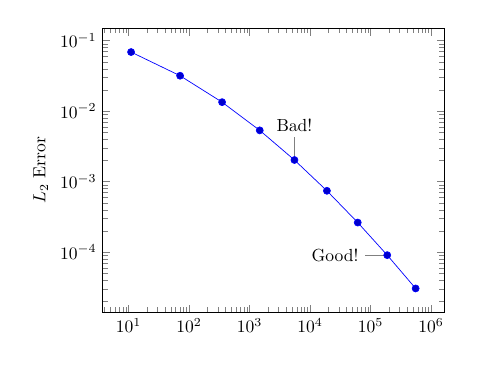
\begin{tikzpicture}[scale = 0.63276]
			\begin{loglogaxis}[
				%xlabel={\textsc{Dof}},
				ylabel={$L_2$ Error},
				]
				\addplot coordinates {
					(11, 6.887e-02)
					(71, 3.177e-02)
					(351, 1.341e-02)
					(1471, 5.334e-03)
					(5503, 2.027e-03)
					(18943, 7.415e-04)
					(61183, 2.628e-04)
					(187903, 9.063e-05)
					(553983, 3.053e-05)
				};
				\node [coordinate,pin=above:{Bad!}]
				at (axis cs:5503,2.027e-03) {};
				\node [coordinate,pin=left:{Good!}]
				at (axis cs:187903,9.063e-05) {};
			\end{loglogaxis}
		\end{tikzpicture}
		\caption{A subfigure}
		\label{fig:sub1}
	\end{subfigure}
	\hfill
	\begin{subfigure}{.49\textwidth}
		\centering
		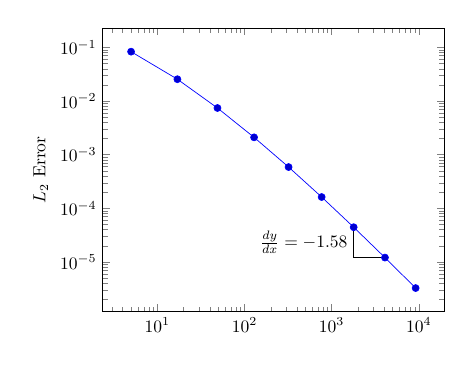
\begin{tikzpicture}[scale = 0.63276]
			\begin{loglogaxis}[
				ylabel=$L_2$ Error,
				]
				\draw
				(1793,4.442e-05)
				|- (4097,1.207e-05)
				node [near start,left]
				{$\frac{dy}{dx} = -1.58$};
				\addplot coordinates {
					(5, 8.312e-02)
					(17, 2.547e-02)
					(49, 7.407e-03)
					(129, 2.102e-03)
					(321, 5.874e-04)
					(769, 1.623e-04)
					(1793, 4.442e-05)
					(4097, 1.207e-05)
					(9217, 3.261e-06)
				};
			\end{loglogaxis}
		\end{tikzpicture}
		\caption{A subfigure}
	  	\label{fig:sub2}
	\end{subfigure}\\

	\begin{subfigure}{.49\textwidth}
		\centering
		\includegraphics[width=.5\linewidth]{\resourcePath eg05}
		\caption{A subfigure}
		\label{fig:sub3}
	\end{subfigure}
	\begin{subfigure}{.49\textwidth}
		\centering
		\includegraphics[width=.5\linewidth]{\resourcePath eg06}
		\caption{A subfigure}
		\label{fig:sub4}
	\end{subfigure}
	\caption{A figure with two subfigures}
	\label{fig:sub}
\end{figure}
 
上面示例中,子圖\ref{fig:sub1}、子圖\ref{fig:sub2}、子圖\ref{fig:sub3}、子圖\ref{fig:sub4}分別表示子圖








\subsubsection{研究動機}
美國學者對公司治理的討論可追溯自1930 年代,Berle \&
Means(1932)指出,美國企業存在著股權分散的必要性,因為隨著企
業規模不斷的擴大,使得多數的中大型公司皆需將經營權與所有權
加以分離來經營,以期達到專業化的目的。
有系統地討論此一問題者為Jensen,在1988 年Jensen 首度有系統地
收錄以公司治理為主題的文章(Weston, Siu \& Johnson; 2002)。







 
\chapter{数学公式}
\begin{equation}
\label{eq1}
e^{\pi i}+1=0
\end{equation}
\begin{align}
2 y & =d\label{eq:IntoSection}\\
3 y & =cx+d\\
4 y_{12} & =bx^{2}+cx+d\\
5 y(x) & =ax^{3}+bx^{2}+cx+d
6 
\end{align}
\begin{equation}
2 x=\left\{ \begin{array}{cl}
3 0 & \textrm{if }A=\ldots\\
4 1 & \textrm{if }B=\ldots\\
5 x & \textrm{this run  text.}\end
{array}\right.
\end{equation}        



有系統\cite{article}地討論此一問題者為Jensen,在1988 年Jensen 首度有系統地
收錄以公司治理為主題的文章(Weston, Siu \& Johnson; 2002)。

美國學者對公司治理的討論可追溯自1930 年代,Berle \&
Means(1932)指出,美國企業存在著股權分散的必要性,因為隨著企
業規模不斷的擴大,使得多數的中大型公司皆需將經營權與所有權
加以分離來經營,以期達到專業化的目的。
有系統地討論此一問題者為Jensen,在1988 年Jensen 首度有系統地
收錄以公司治理為主題的文章(Weston, Siu \& Johnson; 2002)。




\subsection{算法表}
\begin{algorithm}[H]
    \fz[10][0.25]
	\SetAlgoVlined %设置带水平线的连线
	\PrintSemicolon
	\KwData{document set $D :=\{d_1,d_2,\cdots,d_i\}$, term vector $d_1 =\{t_1,t_2,\cdots,t_j\}$
	}
	\KwResult{top6000,High TF-IDF Frequency Keywords}
	\Begin{
	term matrix:$\ \mathcal{L};  \hfill /* \textit{Initial value is empty ($j \times i$)} */$\\
	counter:$\ i =0, j=0;$\\
	    \For{$d  \in D$}{
	        $ i\ $++;\\ 
	        \For {$t \in d$} {
	                $ j\ $ ++;\\[-2mm]
	                $ w_{i,j} = \text{tf}(t,d)\cdot \text{idf}(t,D) = \dfrac{f_{t,d}}{n_d} \cdot \log \dfrac{N}{|\{d \in D: t \in d\}|};$\\
	                $ \mathcal{L}_{i,j}$.Append($t,w_{i,j}$);\\
	            }
            $\mathcal{L}_{i,j}$.Sort(by:$w_{i,j}$)[:10];   \hfill /* \textit{descending rank and retain the top 10.}*/\\
            $\mathcal{L}_{i,j}$.Reindex(); \hfill /* \textit{reset the index.}*/
	        }
   \vspace{-1.5mm} term matrix: $\mathcal{L}= 
    \left[\begin{array}{llll}
    t'_{1,1} & t'_{1,2} & \cdots & t'_{1,10}  \\[-2mm]
    \vdots &\vdots &\vdots & \vdots\\[-1mm]
    t'_{j,1} & t'_{j,2} & \cdots & t'_{j,10}  \\[-1mm]
    \end{array}\right]
    $    \hfill /* \textit{print $\mathcal{L} \ (10\times j)$  result} */\\[0.5em]
    \nlset{Note$^\star$ \ \ \ \ \  }   \textbf{OutputFile: \textbf{File}$^{(1,\divideontimes)}$ } \\[0.5em] 
    \For {$ t' \in \mathcal{L}  $}{
    $i,j \leftarrow t'$ .index()\\[-1mm]
        $w_{i,j} = \text{tf}(t', \mathcal{L}  ) =  \dfrac{f_{t'} }{10 \cdot j} ;$           \hfill /* \textit{where $f_{t'}$ is the raw count of a term $t'$ in $\mathcal{L} $ }*/ \\
    }
     \nlset{Remark$^\star$ \ \ \ \ \  }  $\mathcal{L} $.Sort(by:$w_{i,j}$)[:6000];   \hfill /* \textit{descending rank and retain the top 6000.}*/\\[0.5em]
         \nlset{Note$^\star$ \ \ \ \ \  }   \textbf{OutputFile: \textbf{File}$^{(2,\divideontimes)}$ }  \\[0.5em]
    \textbf{End}
    }	
	\caption{Text Mining: Keyword Extraction Algorithm}
\end{algorithm}

 











% 请确保bib 文件名称为 ref.bib, 利用js文件处理后的bbl文件名称为 ref.bbl
\addreference














\begin{appendix}
證明過程
\end{appendix}











\begin{acknowpage}
谢谢各位
\end{acknowpage}









 
\begin{addcvpage}
% 設置入學時間
\addedudate{2019 年 7 月}




% 填寫教育經歷,注意內容以逗号作分隔,
\addeduItem{2009.16-2012.13,中国澳门氹仔岛澳门科技大学,商學院}
\addeduItem{2009.16-2012.13,澳门科技大学,商学院}
\addeduItem{2009.16-2012.13,澳门科技大学,商学院}



%增加學術文章
\addpaperItem{ 
    \item 中国澳门氹仔岛澳门科技大学1中国澳门氹仔岛澳门科技大学1中国澳门氹仔岛澳门科技大学1中国澳门氹仔岛澳门科技大学1中国澳门氹仔岛澳门科技大学1中国澳门氹仔岛澳门科技大学1中国澳门氹仔岛澳门科技大学1中国澳门氹仔岛澳门科技大学,
    \item 中国澳门氹仔岛澳门科技大学,
}




% 增加項目
\addprojectItem{
    \item 中国澳门氹仔岛澳门科技大学,商学院商学院
    \item  商学院商学院商学院中国澳门氹仔岛澳门科技大学,商学院商学院商学院商学院商学院中国澳门氹仔岛澳门科技大学,商学院商学院商学院商学院商学院
}
\end{addcvpage}











\end{document}